% ARTICLE ----
% This is just here so I know exactly what I'm looking at in Rstudio when messing with stuff.
\documentclass[11pt,]{article}
\usepackage[left=1in,top=1in,right=1in,bottom=1in]{geometry}
\newcommand*{\authorfont}{\fontfamily{phv}\selectfont}
\usepackage[]{mathpazo}


  \usepackage[T1]{fontenc}
  \usepackage[utf8]{inputenc}




\usepackage{abstract}
\renewcommand{\abstractname}{}    % clear the title
\renewcommand{\absnamepos}{empty} % originally center

\renewenvironment{abstract}
 {{%
    \setlength{\leftmargin}{0mm}
    \setlength{\rightmargin}{\leftmargin}%
  }%
  \relax}
 {\endlist}

\makeatletter
\def\@maketitle{%
  \newpage
%  \null
%  \vskip 2em%
%  \begin{center}%
  \let \footnote \thanks
    {\fontsize{18}{20}\selectfont\raggedright  \setlength{\parindent}{0pt} \@title \par}%
}
%\fi
\makeatother




\setcounter{secnumdepth}{0}

\usepackage{color}
\usepackage{fancyvrb}
\newcommand{\VerbBar}{|}
\newcommand{\VERB}{\Verb[commandchars=\\\{\}]}
\DefineVerbatimEnvironment{Highlighting}{Verbatim}{commandchars=\\\{\}}
% Add ',fontsize=\small' for more characters per line
\usepackage{framed}
\definecolor{shadecolor}{RGB}{248,248,248}
\newenvironment{Shaded}{\begin{snugshade}}{\end{snugshade}}
\newcommand{\AlertTok}[1]{\textcolor[rgb]{0.94,0.16,0.16}{#1}}
\newcommand{\AnnotationTok}[1]{\textcolor[rgb]{0.56,0.35,0.01}{\textbf{\textit{#1}}}}
\newcommand{\AttributeTok}[1]{\textcolor[rgb]{0.13,0.29,0.53}{#1}}
\newcommand{\BaseNTok}[1]{\textcolor[rgb]{0.00,0.00,0.81}{#1}}
\newcommand{\BuiltInTok}[1]{#1}
\newcommand{\CharTok}[1]{\textcolor[rgb]{0.31,0.60,0.02}{#1}}
\newcommand{\CommentTok}[1]{\textcolor[rgb]{0.56,0.35,0.01}{\textit{#1}}}
\newcommand{\CommentVarTok}[1]{\textcolor[rgb]{0.56,0.35,0.01}{\textbf{\textit{#1}}}}
\newcommand{\ConstantTok}[1]{\textcolor[rgb]{0.56,0.35,0.01}{#1}}
\newcommand{\ControlFlowTok}[1]{\textcolor[rgb]{0.13,0.29,0.53}{\textbf{#1}}}
\newcommand{\DataTypeTok}[1]{\textcolor[rgb]{0.13,0.29,0.53}{#1}}
\newcommand{\DecValTok}[1]{\textcolor[rgb]{0.00,0.00,0.81}{#1}}
\newcommand{\DocumentationTok}[1]{\textcolor[rgb]{0.56,0.35,0.01}{\textbf{\textit{#1}}}}
\newcommand{\ErrorTok}[1]{\textcolor[rgb]{0.64,0.00,0.00}{\textbf{#1}}}
\newcommand{\ExtensionTok}[1]{#1}
\newcommand{\FloatTok}[1]{\textcolor[rgb]{0.00,0.00,0.81}{#1}}
\newcommand{\FunctionTok}[1]{\textcolor[rgb]{0.13,0.29,0.53}{\textbf{#1}}}
\newcommand{\ImportTok}[1]{#1}
\newcommand{\InformationTok}[1]{\textcolor[rgb]{0.56,0.35,0.01}{\textbf{\textit{#1}}}}
\newcommand{\KeywordTok}[1]{\textcolor[rgb]{0.13,0.29,0.53}{\textbf{#1}}}
\newcommand{\NormalTok}[1]{#1}
\newcommand{\OperatorTok}[1]{\textcolor[rgb]{0.81,0.36,0.00}{\textbf{#1}}}
\newcommand{\OtherTok}[1]{\textcolor[rgb]{0.56,0.35,0.01}{#1}}
\newcommand{\PreprocessorTok}[1]{\textcolor[rgb]{0.56,0.35,0.01}{\textit{#1}}}
\newcommand{\RegionMarkerTok}[1]{#1}
\newcommand{\SpecialCharTok}[1]{\textcolor[rgb]{0.81,0.36,0.00}{\textbf{#1}}}
\newcommand{\SpecialStringTok}[1]{\textcolor[rgb]{0.31,0.60,0.02}{#1}}
\newcommand{\StringTok}[1]{\textcolor[rgb]{0.31,0.60,0.02}{#1}}
\newcommand{\VariableTok}[1]{\textcolor[rgb]{0.00,0.00,0.00}{#1}}
\newcommand{\VerbatimStringTok}[1]{\textcolor[rgb]{0.31,0.60,0.02}{#1}}
\newcommand{\WarningTok}[1]{\textcolor[rgb]{0.56,0.35,0.01}{\textbf{\textit{#1}}}}

% --------------------------------
% Separating this because this no
% longer works as of pandoc 3.2.1
% -------------------------------
%%\usepackage{graphicx,grffile}
%\makeatletter
%\def\maxwidth{\ifdim\Gin@nat@width>\linewidth\linewidth\else\Gin@nat@width\fi}
%\def\maxheight{\ifdim\Gin@nat@height>\textheight\textheight\else\Gin@nat@height\fi}
%\makeatother
%% Scale images if necessary, so that they will not overflow the page
%% margins by default, and it is still possible to overwrite the defaults
%% using explicit options in \includegraphics[width, height, ...]{}
%\setkeys{Gin}{width=\maxwidth,height=\maxheight,keepaspectratio}
%
% ---------------------------------
% This works now: HT: Justin Esarey
% ---------------------------------
\usepackage{graphicx}
\makeatletter
\newsavebox\pandoc@box
\newcommand*\pandocbounded[1]{% scales image to fit in text height/width
  \sbox\pandoc@box{#1}%
  \Gscale@div\@tempa{\textheight}{\dimexpr\ht\pandoc@box+\dp\pandoc@box\relax}%
  \Gscale@div\@tempb{\linewidth}{\wd\pandoc@box}%
  \ifdim\@tempb\p@<\@tempa\p@\let\@tempa\@tempb\fi% select the smaller of both
  \ifdim\@tempa\p@<\p@\scalebox{\@tempa}{\usebox\pandoc@box}%
  \else\usebox{\pandoc@box}%
  \fi%
}
% Set default figure placement to htbp
\def\fps@figure{htbp}
\makeatother

% ^ saving this note in case I want some kind of conditional operation thingie.


\title{Resultados preliminares  }



\author{\Large Caio Gomes
Alves\vspace{0.05in} \newline\normalsize\emph{Instituto de Matemática,
Estatística e Computação Científica - UNICAMP}  }


\date{}

\usepackage{titlesec}

\titleformat*{\section}{\normalsize\bfseries}
\titleformat*{\subsection}{\normalsize\itshape}
\titleformat*{\subsubsection}{\normalsize\itshape}
\titleformat*{\paragraph}{\normalsize\itshape}
\titleformat*{\subparagraph}{\normalsize\itshape}


\usepackage{natbib}
\bibliographystyle{apsr}
\usepackage[strings]{underscore} % protect underscores in most circumstances



\newtheorem{hypothesis}{Hypothesis}
\usepackage{setspace}


% set default figure placement to htbp
\makeatletter
\def\fps@figure{htbp}
\makeatother


% move the hyperref stuff down here, after header-includes, to allow for - \usepackage{hyperref}

\makeatletter
\@ifpackageloaded{hyperref}{}{%
\ifxetex
  \PassOptionsToPackage{hyphens}{url}\usepackage[setpagesize=false, % page size defined by xetex
              unicode=false, % unicode breaks when used with xetex
              xetex]{hyperref}
\else
  \PassOptionsToPackage{hyphens}{url}\usepackage[draft,unicode=true]{hyperref}
\fi
}

\@ifpackageloaded{color}{
    \PassOptionsToPackage{usenames,dvipsnames}{color}
}{%
    \usepackage[usenames,dvipsnames]{color}
}
\makeatother
\hypersetup{breaklinks=true,
            bookmarks=true,
            pdfauthor={Caio Gomes Alves (Instituto de Matemática,
Estatística e Computação Científica - UNICAMP)},
             pdfkeywords = {},
            pdftitle={Resultados preliminares},
            colorlinks=true,
            citecolor=blue,
            urlcolor=blue,
            linkcolor=magenta,
            pdfborder={0 0 0}}
\urlstyle{same}  % don't use monospace font for urls

% Add an option for endnotes. -----


% add tightlist ----------
\providecommand{\tightlist}{%
\setlength{\itemsep}{0pt}\setlength{\parskip}{0pt}}

% add some other packages ----------

% \usepackage{multicol}
% This should regulate where figures float
% See: https://tex.stackexchange.com/questions/2275/keeping-tables-figures-close-to-where-they-are-mentioned
\usepackage[section]{placeins}

% CSL environment change -----


% Last minute stuff -----
\usepackage{amssymb,amsmath} % HT @ashenkin


\begin{document}

% \pagenumbering{arabic}% resets `page` counter to 1
%
% \maketitle

{% \usefont{T1}{pnc}{m}{n}
\setlength{\parindent}{0pt}
\thispagestyle{plain}
{\fontsize{18}{20}\selectfont\raggedright
\maketitle  % title \par

}

{
   \vskip 13.5pt\relax \normalsize\fontsize{11}{12}
\textbf{\authorfont Caio Gomes Alves} \hskip 15pt \emph{\small Instituto
de Matemática, Estatística e Computação Científica - UNICAMP}   

}

}






\vskip -8.5pt


 % removetitleabstract

\noindent 

\hypertarget{mudanuxe7as-na-modelagem}{%
\section{Mudanças na modelagem}\label{mudanuxe7as-na-modelagem}}

\hypertarget{parametrizauxe7uxe3o}{%
\subsection{Parametrização}\label{parametrizauxe7uxe3o}}

Para que a comparação entre o método proposto e o já existente pelo
pacote \texttt{ETAS} seja mais direta, a parametrização do modelo foi
ajustada para seguir a de \cite{Jalilian_2019}, como segue:

\begin{equation}
\lambda_{\theta}(t,x,y|\mathcal{H}_{t}) = \mu(x,y) + \sum_{i: t_{i} < t}\kappa_{A,\alpha}(m_{i})g_{c,p}(t - t_{i})f_{D,\gamma,q}(x - x_{i}, y - y_{i}, m_{i})
\end{equation}

Onde:

\begin{align*}
\kappa_{A,\alpha}(m_{i}) &= A \, \mathrm{exp}\left(\alpha(m_{i} - m_{0})\right) \\ \\
g_{c,p}(t - t_{i}) &= \frac{p-1}{c}\left(1 + \frac{t - t_{i}}{c}\right)^{-p} \\ \\
f_{D,\gamma,q}(x - x_{i},y - y_{i}; m_{i}) &= \frac{q - 1}{\pi D \mathrm{exp}\left(\gamma(m_{i} - m_{0})\right)}\left(1 + \frac{(x - x_{i})^{2} + (y - y_{i})^{2}}{D \mathrm{exp}\left(\gamma(m_{i} - m_{0})\right)}\right)
\end{align*}

Assim, tanto a produtividade \(\kappa(m_{i})\) quanto a distribuição da
Lei de Omori Modificada \(g(t - t_{i})\) seguem as mesmas
parametrizações anteriores, mudando a distribuição espacial dos
\emph{aftershocks} para uma radialmente simétrica e isotrópica
\(f(x - x_{i}, y - y_{i};m_{i})\), como proposta por \cite{Ogata_1988}.
O \emph{background rate} \(\mu(x,y)\) é estimado de maneira
semi-paramétrica, por um \emph{kernel} adaptativo e condicional às
probabilidades de ser pai/filho.

Uma diferença para o que é feito pelo pacote \texttt{ETAS} é que o mesmo
considera a distribuição das magnitudes (marcas) como seguindo uma
distribuição exponencial com parâmetro \(\beta\) a ser estimada. No
método proposto, é considerada a Lei de Gutenberg-Richter e a
modificação de Utsu, como segue:

\begin{align*}
\log_{10}(N) &= a - b \times m \\
\hat{b} &= \frac{\log_{10}(e)}{\left(\bar{m} - m_{0}\right)}
\end{align*}

Onde \(a\) é uma constante não que não precisa ser estimada, \(\bar{m}\)
é a média das magnitudes maiores do que \(m_{0}\) no catálogo, enquanto
que \(\hat{b}\) é estimado de maneira separada dos demais parâmetros do
modelo (devido à independência das marcas que é suposição do modelo).

A log-verossimilhança do modelo foi implementada pela função
\texttt{log_lik_etas} e depende das probabilidades de ser pai/filho,
estimadas no passo E. O gradiente da log-verossimilhança também foi
implementado e atualizado para incluir os novos parâmetros, por meio da
função \texttt{gradiente_etas_completo}. Ambos são usados no passo M,
por meio da função \texttt{optim}, utilizando o método L-BFGS-B que
impõe restrições de caixa para que não ocorram escapes do espaço
paramétrico.

\hypertarget{otimizauxe7uxe3o-do-cuxe1lculo-de-probabilidades}{%
\subsection{Otimização do cálculo de
probabilidades}\label{otimizauxe7uxe3o-do-cuxe1lculo-de-probabilidades}}

O cálculo principal do passo E do algoritmo EM implementado se dá por
meio das seguintes contas:

\begin{align*}
p_{i,j} &= \begin{cases}
\frac{\kappa(m_{i})g(t_{j} - t_{i})f(x_{j} - x_{i},y_{j} - y_{i};m_{i})}{\lambda_{\theta}(t_{j},x_{j},y_{j}|\mathcal{H}_{t_{j}})}, & t_{j} > t_{i} \\
0 & t_{j} \le t_{i}
\end{cases} \\
p_{j} &= \sum_{i: t_{i} < t_{j}}p_{i,j}, \,\,\, j = 1,\ldots,N
\end{align*}

Que calcula a probabilidade \(p_{i,j}\) de um evento \(j\) ser filho de
um evento \(i\), e a probabilidade \(p_{j}\) de um evento ser filho
independentemente de quem seja o pai. Anteriormente, a função
implementada (\texttt{calcular_probabilidades}) fazia a chamada de
funções externas repetidamente, sendo que a mesma podia ser feita apenas
uma vez. A nova implementação está como segue:

\begin{Shaded}
\begin{Highlighting}[]
\CommentTok{\# Calcula as probabilidades p\_ij (passo E do EM):}
\NormalTok{calcular\_probabilidades }\OtherTok{\textless{}{-}} \ControlFlowTok{function}\NormalTok{(df\_eventos, theta, M0, raster\_mu,}
\NormalTok{                                    x\_grid, y\_grid, }\AttributeTok{num\_cores =} \DecValTok{1}\NormalTok{) \{}
\NormalTok{    n }\OtherTok{\textless{}{-}} \FunctionTok{nrow}\NormalTok{(df\_eventos)}
    \CommentTok{\# Valores do background rate (mu) para todos os eventos:}
\NormalTok{    mu\_vals }\OtherTok{\textless{}{-}} \FunctionTok{func\_nu}\NormalTok{(raster\_mu, df\_eventos, x\_grid, y\_grid)}\SpecialCharTok{$}\NormalTok{lyr}\FloatTok{.1}
    \CommentTok{\# Cálculo paralelizado pelo mclapply:}
\NormalTok{    probabilidades }\OtherTok{\textless{}{-}} \FunctionTok{mclapply}\NormalTok{(}\DecValTok{1}\SpecialCharTok{:}\NormalTok{n, }\ControlFlowTok{function}\NormalTok{(j) \{}
        \CommentTok{\# Primeiro evento tem probabilidade 0 de ser descendente:}
        \ControlFlowTok{if}\NormalTok{ (j }\SpecialCharTok{==} \DecValTok{1}\NormalTok{) }\FunctionTok{return}\NormalTok{(}\FunctionTok{numeric}\NormalTok{(}\DecValTok{0}\NormalTok{))}
        \CommentTok{\# Atualiza o índice de cada evento:}
\NormalTok{        i\_indices }\OtherTok{\textless{}{-}} \DecValTok{1}\SpecialCharTok{:}\NormalTok{(j }\SpecialCharTok{{-}} \DecValTok{1}\NormalTok{)}
\NormalTok{        numeradores }\OtherTok{\textless{}{-}} \FunctionTok{kappa\_func}\NormalTok{(df\_eventos}\SpecialCharTok{$}\NormalTok{mag[i\_indices], M0, theta[}\StringTok{"A"}\NormalTok{], theta[}\StringTok{"alpha"}\NormalTok{]) }\SpecialCharTok{*}
            \FunctionTok{g\_func}\NormalTok{(df\_eventos}\SpecialCharTok{$}\NormalTok{time[j] }\SpecialCharTok{{-}}\NormalTok{ df\_eventos}\SpecialCharTok{$}\NormalTok{time[i\_indices], theta[}\StringTok{"c"}\NormalTok{], theta[}\StringTok{"p"}\NormalTok{]) }\SpecialCharTok{*}
            \FunctionTok{f\_spatial}\NormalTok{(}
\NormalTok{            (df\_eventos}\SpecialCharTok{$}\NormalTok{x[j] }\SpecialCharTok{{-}}\NormalTok{ df\_eventos}\SpecialCharTok{$}\NormalTok{x[i\_indices])}\SpecialCharTok{\^{}}\DecValTok{2} \SpecialCharTok{+}
\NormalTok{            (df\_eventos}\SpecialCharTok{$}\NormalTok{y[j] }\SpecialCharTok{{-}}\NormalTok{ df\_eventos}\SpecialCharTok{$}\NormalTok{y[i\_indices])}\SpecialCharTok{\^{}}\DecValTok{2}\NormalTok{,}
\NormalTok{            df\_eventos}\SpecialCharTok{$}\NormalTok{mag[i\_indices], M0, theta[}\StringTok{"D"}\NormalTok{], theta[}\StringTok{"q"}\NormalTok{], theta[}\StringTok{"gamma"}\NormalTok{]}
\NormalTok{            )}
\NormalTok{        denom }\OtherTok{\textless{}{-}}\NormalTok{ mu\_vals[j] }\SpecialCharTok{+} \FunctionTok{sum}\NormalTok{(numeradores)}
        \FunctionTok{return}\NormalTok{(numeradores }\SpecialCharTok{/}\NormalTok{ denom)}
\NormalTok{    \}, }\AttributeTok{mc.cores =}\NormalTok{ num\_cores)}
\NormalTok{    prob\_total }\OtherTok{\textless{}{-}} \FunctionTok{vapply}\NormalTok{(probabilidades, sum, }\FunctionTok{numeric}\NormalTok{(}\DecValTok{1}\NormalTok{))}
    \CommentTok{\# Retorna as probabilidades individuais e totais de cada evento:}
    \FunctionTok{list}\NormalTok{(}\AttributeTok{probabilidades =}\NormalTok{ probabilidades, }\AttributeTok{prob\_total =}\NormalTok{ prob\_total)}
\NormalTok{\}}
\end{Highlighting}
\end{Shaded}

Com a nova implementação, o tempo necessário para calcular o passo E foi
reduzido drasticamente, acelerando assim o processo de modelagem como um
todo.

\hypertarget{anuxe1lise-de-resuxedduos}{%
\section{Análise de Resíduos}\label{anuxe1lise-de-resuxedduos}}

Podemos verificar a qualidade do ajuste realizado por meio dos resíduos
do modelo. Para isso, avaliam-se duas dimensões: temporal e espacial. A
partir de agora, todas as análises serão feitas para o catálogo do Irã,
usado por Jalilian no artigo do pacote \texttt{etas}.

\hypertarget{temporais}{%
\subsection{Temporais}\label{temporais}}

Para a parte temporal, podemos usar a intensidade condicional temporal
que é dada pela integral da intensidade completa no espaço, que é dada
por:

\begin{equation}
\int_{0}^{\Delta t}g(s)\, ds = 1 - \left(\frac{c}{\Delta t + c}\right)^{p - 1}
\end{equation}

Podemos assim calcular \(\tau\) (a intensidade acumulada) para qualquer
tempo, por meio da função \texttt{calcular_tau}. Sejam os tempos de dois
eventos seguidos \(t_{i}\) e \(t_{j}\), então
\(\tau_{i,j} = \int_{t_{i}}^{t_{j}}g(s)\, ds = 1 - \left(\frac{c}{(t_{j} - t_{i}) + c}\right)^{p-1}\).
Se o modelo estiver bem ajustado (no sentido dos parâmetros temporais
\(c\) e \(p\)), então \(U_{i,j} = 1 - \exp(-\tau_{i,j})\), com
\(U \sim \mathrm{Unif}(0,1)\).

Com os valores ajustados (0.160274, 1.2817266), teremos que:

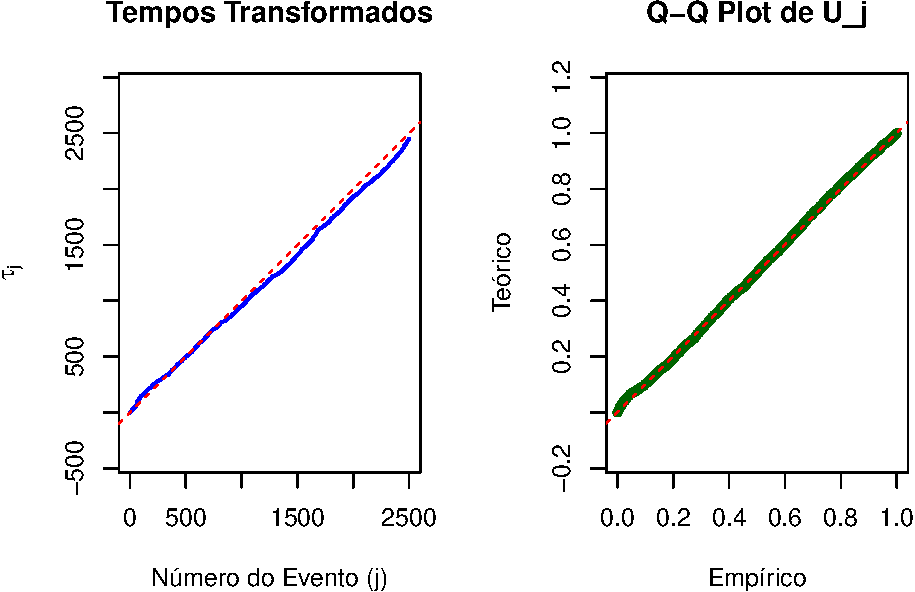
\includegraphics{relatorio_1_files/relatorio_1_files/figure-latex/resid_temp-1.pdf}

Podemos ver que os tempos transformados e o Q-Q Plot apresentam ajustes
ótimos, podendo ser feito o teste de Kolmogorov-Smirnov para testar se
\(U_{j}\) é uniformemente distribuído:

\begin{verbatim}
## 
##  Asymptotic one-sample Kolmogorov-Smirnov test
## 
## data:  U_j_iran
## D = 0.020431, p-value = 0.2476
## alternative hypothesis: two-sided
\end{verbatim}

Além disso, podemos fazer uma análise de resíduos por \emph{bins}. Isso
é feito por meio da diferença entre a quantidade de terrremotos
ocorridos em cada intervalo e a quantidade esperada dada pelo modelo
(calculada da mesma forma que anteriormente, porém com os limites sendo
os de cada intervalo). Após isso, para serem normalizados, divide-se
pela raiz quadrada da quantidade esperada e, caso o modelo esteja bem
ajustado, não deve pode aparentar nenhuma forma de padrão temporal. Para
100 \emph{bins}, teremos:

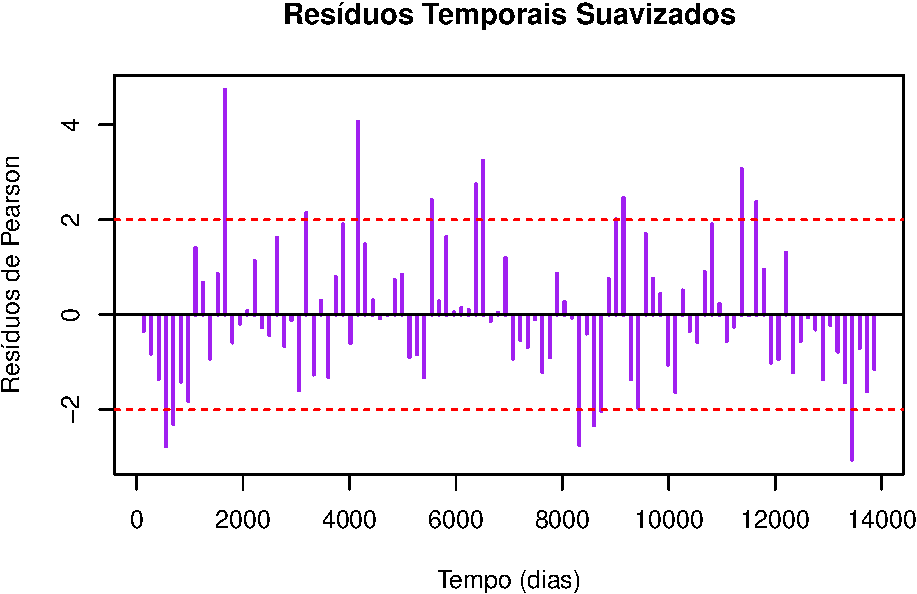
\includegraphics{relatorio_1_files/relatorio_1_files/figure-latex/resid_temp_bin-1.pdf}

\hypertarget{espaciais}{%
\subsection{Espaciais}\label{espaciais}}

A mesma ideia é feita para a dimensão espacial, sendo avaliada a
diferença entre a quantidade de terremotos ocorridos em um \emph{pixel}
no \emph{grid} da região de interesse, e a quantidade esperada dada pelo
modelo. Para isso, é necessário criar a densidade espacial esperada
gerada pelo \emph{background rate} (que depende da probabilidade de ser
pai/filho estimada pelo passo E do EM), que é dependente somente dos
pais.

Após isso, todos os eventos contribuem para a intensidade condicional,
usando os parâmetros estimados pelo modelo. Com isso, temos que a
quantidade esperada pelo modelo será dada pela soma da contribuição do
\emph{background} com a intensidade condicional de cada evento.

Caso o modelo esteja bem ajustado, não deve ser possível identificar
nenhuma forma de padrão espacialmente distribuído. Os resultados são os
seguintes:

\begin{center}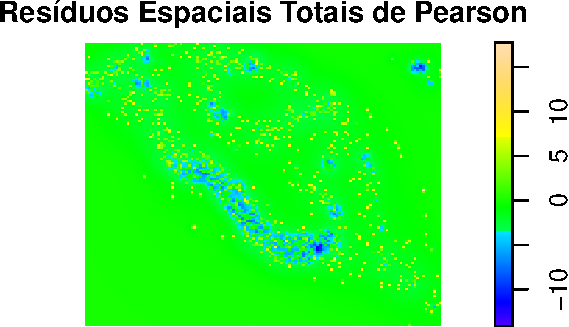
\includegraphics{relatorio_1_files/figure-latex/resid_espac-1} \end{center}

Há regiões em que ocorreram eventos mas com pouca quantidade esperada
(dada pelos pontos amarelos), enquanto que há uma região com valores
esperados altos, mas poucos eventos ocorridos. Isso provavelmente ocorre
pelo tamanho do \emph{grid} (feito em 128 por 128 \emph{pixels}), que
caso fosse menor não teria uma região com subestimação.

\hypertarget{erro-padruxe3o-dos-estimadores}{%
\section{Erro-padrão dos
estimadores}\label{erro-padruxe3o-dos-estimadores}}

\hypertarget{via-hessiana}{%
\subsection{Via Hessiana}\label{via-hessiana}}

Como o gradiente da função de log-verossimilhança é dado para o
\texttt{optim()}, ao final da otimização o valor da hessiana pode ser
extraído, e pelo fato da verossimilhança ser fatorável, o resultado é
uma matriz hessiana \(\hat{H}_{\theta}\) bloco-diagonal, com parâmetros
que não tem correlação tendo valor 0.

Assim, o erro-padrão de cada estimativa pode ser calculado de forma:

\begin{equation}
EP(\theta) = \sqrt{\mathrm{diag}\left(\hat{H}_{\theta}^{-1}\right)}
\end{equation}

Para o catálogo do Irã (usado para título de comparação entre o método
proposto e o de \cite{Jalilian_2019}), temos que a hessiana ao final do
último passo é:

\begin{verbatim}
##               A     alpha         c         p           D           q      gamma
## A     18752.891 1535.7208     0.000     0.000       0.000      0.0000    0.00000
## alpha  1535.721  240.6471     0.000     0.000       0.000      0.0000    0.00000
## c         0.000    0.0000  3802.513 -4764.767       0.000      0.0000    0.00000
## p         0.000    0.0000 -4764.767 12331.984       0.000      0.0000    0.00000
## D         0.000    0.0000     0.000     0.000 1054134.952 -25391.8841 6864.20288
## q         0.000    0.0000     0.000     0.000  -25391.884    785.6389 -165.56879
## gamma     0.000    0.0000     0.000     0.000    6864.203   -165.5688   86.68414
\end{verbatim}

Vale notar que a mesma é realmente bloco-diagonal, como esperado pela
forma da verossimilhança. O erro-padrão estimado para cada parâmetro,
junto com o valor estimado, será:

\begin{verbatim}
##                      A      alpha         c          p           D          q      gamma
## Estimativas 0.22846076 1.94867209 0.1602740 1.28172658 0.018228922 2.11616976 0.04525585
## Erro-Padrão 0.01056886 0.09329789 0.0225789 0.01253781 0.002298591 0.07580962 0.15432858
\end{verbatim}

Os valores usados como chute inicial foram
\(\theta = (A = 0.23, \alpha = 2.8, c = 0.022, p = 1.12, D = 0.012, q = 2.3, \gamma = 0.03)\),
que são os mesmos usados no \emph{paper} \cite{Jalilian_2019}. Para
título de comparação, os valores das estimativas e erros-padrões
associados quando usada a função \texttt{etas} são:

\begin{verbatim}
## ETAS model: fitted using iterative stochastic declustering method
## converged after 5 iterations: elapsed execution time 8.78 minutes
## 
## ML estimates of model parameters:
##            beta     mu      A      c  alpha      p      D      q     gamma
## Estimate 5.8043 0.5134 0.1883 0.0595 2.3269 1.1692 0.0226 2.6492         0
## StdErr   0.0297 0.0098 0.0371 0.0876 0.0333 0.0083 0.0824 0.0372 164193441
## 
## Declustering probabilities:
##    Min. 1st Qu.  Median    Mean 3rd Qu.    Max. 
##  0.0000  0.1069  0.9094  0.6414  0.9796  1.0000 
## 
## log-likelihood:  -7146.193   AIC:  14308.39
\end{verbatim}

Podemos ver que os valores estimados por ambos os métodos foram
(relativamente) próximos, mas com erros-padrões muito diferentes.

\hypertarget{via-bootstrap}{%
\subsection{\texorpdfstring{Via
\emph{bootstrap}}{Via bootstrap}}\label{via-bootstrap}}

Vale citar que a estimativa do erro-padrão dos estimadores obtida por
meio da hessiana do passo M subestima a verdadeira variabilidade, como
demonstrada por \cite{Louis_1982}. Isso ocorre pois a quantidade de
observações efetiva é menor do que a usada para maximizar a função
objetivo, que usa a verossimilhança completa ao invés da parcial.

Uma forma de ``prevenir'' esse problema seria simular várias amostras
\emph{bootstrap} de catálogos usando os valores estimados pelo modelo
(tanto de \emph{background rate} quanto de \(\hat{\theta}\)), reajustar
o modelo para cada uma das amostras, e utilizar os resultados para
calcular o erro-padrão \emph{bootstrap} (além de outras quantidades,
como viés e intervalos de confiança \emph{bootstrap}).

Por isso, um estudo de simulação foi feito, com 100 amostras
\emph{bootstrap} geradas a partir das estimativas finais de
\(\hat\mu(x,y)\) e \(\hat{\theta}\), com diferentes sementes, utilizando
\(\hat{b} = 2\) (aproximadamente o valor estimado para a Lei de
Gutenberg-Richter, dado por \(2.009878\)) e a função
\texttt{simular_catalogo_etas}. Para cada uma das \(b = 1,\ldots,100\)
amostras o valor de \(\hat{\theta}^{(b)}\) foi extraído, juntamente com
o \(\hat{\mu}(x,y)^{(b)}\). Todas convergiram após 11 a 18 iterações,
sem nenhuma falha.

Os valores dos erro-padrão e viés \emph{bootstrap} são dados por:

\begin{verbatim}
##                 A       alpha          c          p           D          q      gamma
## Est    0.22846076  1.94867209 0.16027401 1.28172658 0.018228922 2.11616976 0.04525585
## EP     0.01056886  0.09329789 0.02257890 0.01253781 0.002298591 0.07580962 0.15432858
## EPB    0.02172104  0.26890268 0.07639258 0.03969417 0.006976795 0.25871173 0.29088490
## ViésB -0.02084282 -0.02381726 0.12157495 0.15556951 0.002124040 0.11351159 0.13643373
\end{verbatim}

As duas primeiras linhas são os valores estimados pelo modelo e seu
erro-padrão usual (calculado via hessiana). Podemos ver que para todos
os parâmetros, o erro-padrão \emph{bootstrap} é maior do que o usual. Os
intervalos de confiança \emph{bootstrap} serão:

\begin{verbatim}
##               A    alpha         c        p          D        q        gamma
## 2.5%  0.1707297 1.313721 0.1715007 1.366028 0.01065099 1.839206 0.0000000001
## 97.5% 0.2506438 2.375211 0.4393014 1.512546 0.03665571 2.844442 0.9022696682
\end{verbatim}

Para \(\gamma\) ocorre um problema em que muitas simulações geraram
valores de terremotos muito próximos do limiar (\(m_{0} = 4.5\)), de
modo que o modelo não detecta influência das magnitudes no aumento de
dispersão espacial dos \emph{aftershocks}. Assim, o quantil 2.5\% desse
parâmetro captura o limiar do espaço paramétrico do \texttt{optim}
(definido em 10\^{}\{-10\}).

\hypertarget{prediuxe7uxe3o}{%
\section{Predição}\label{prediuxe7uxe3o}}

Para a predição de eventos futuros (algo complicado de ser feito, como
explicitado em \cite{Veen_2008}, \cite{Ogata_1988} e \cite{Ogata_1998},
por exemplo), podemos usar uma metodologia baseada na simulação de
catálogos futuros, condicional ao histórico dado pelo catálogo real, ao
\emph{background rate} estimado e ao conjunto de parâmetros obtidos pelo
modelo.

Com esse método, é gerado um catálogo ``expandido'', com os eventos já
ocorridos e novos que ocorrem após o tempo final \(T\). Geram-se várias
simulações, cada uma gerando uma possível realização do futuro, e
agrega-se os valores temporal/espacialmente, para serem feitas predições
do tipo: quantos eventos ocorrerão em \([T, T + \Delta t]\), e onde os
mesmos possuem maiores chances de ocorrência.

Foi implementada uma função chamada \texttt{simular_previsao_etas} que
realiza esse processo utilizando o catálogo passado,
\(\hat{\mu}(x,y), \hat{\theta}\) e um valor de horizonte (quantos dias
serão simulados após o tempo final \(T\)). Outra função foi
implementada, chamada \texttt{gerar_previsoes_etas}, recebendo os mesmos
objetos e usando \texttt{simular_previsao_etas} internamente. O valor de
\(\hat{\theta}\) usado pode ser um único vetor (para a estimativa
pontual, por exemplo), ou uma lista de vetores (para as réplicas
\emph{bootstrap}, por exemplo), que é sorteada em cada simulação. Dessa
forma, é possível propagar a incerteza da estimação de \(\hat{\theta}\)
na predição, aproveitando os valores obtidos no estudo de simulação.

As predições (temporais e espaciais) são posteriormente agregadas usando
as funções \texttt{agregar_previsao_temporal} e
\texttt{agregar_previsao_espacial}, que extraem as informações de cada
uma das simulações e retornam estatísticas como:

\begin{itemize}
\tightlist
\item
  Quantidade média de eventos por período de tempo (deixei 30 dias por
  padrão, para predição a nível de meses), bem como mediana e percentis
  (2.5\% e 97.5\%);
\item
  Contagem média de eventos por célula/\emph{pixel} do \emph{grid} de
  interesse, bem como a probabilidade de que ao menos um evento tenha
  ocorrido na célula (calculada de maneira empírica, usando que
  \(P(N_{\mathrm{celula}} \ge 1) = 1 - \exp(-\hat{\lambda}_{\mathrm{celula}})\),
  com \(\hat{\lambda}_{celula}\) sendo estimada como a contagem média na
  célula).
\end{itemize}

\hypertarget{usando-um-uxfanico-theta}{%
\subsection{\texorpdfstring{Usando um único
\(\theta\)}{Usando um único \textbackslash theta}}\label{usando-um-uxfanico-theta}}

Para o catálogo de terremotos no Irã, simulei 1.000 predições após o
tempo final, usando os valores de \(\hat{\theta}\) (0.2284608,
1.9486721, 0.160274, 1.2817266, 0.0182289, 2.1161698, 0.0452558), em um
horizonte de 210 dias (7 meses). Os valores temporais agregados para os
210 dias, mês a mês foram:

\begin{verbatim}
##   bin_inicio  bin_fim media mediana  p025 p975
## 1   13873.35 13903.35 4.808       4 0.000   13
## 2   13903.35 13933.35 5.060       5 1.000   13
## 3   13933.35 13963.35 4.954       4 1.000   12
## 4   13963.35 13993.35 5.077       5 1.000   12
## 5   13993.35 14023.35 5.093       5 0.975   12
## 6   14023.35 14053.35 5.008       4 1.000   12
## 7   14053.35 14083.35 5.095       5 1.000   12
\end{verbatim}

Ou seja, a quantidade média esperada para cada mês é de aproximadamente
5 eventos/mês (o valor observado pelo catálogo completo é de
aproximadamente 5.40 eventos/mês, com os últimos 12 meses tendo (2, 8,
5, 3, 3, 2, 3, 3, 3, 5, 0, 7, 1) eventos). Ou seja, a predição foi capaz
de capturar o comportamento da quantidade de eventos ocorrendo em
períodos de tempo futuros ao fim do período de observação.

Para a predição espacial, temos que o mapa da contagem média por célula
e a probabilidade de ao menos um evento será:

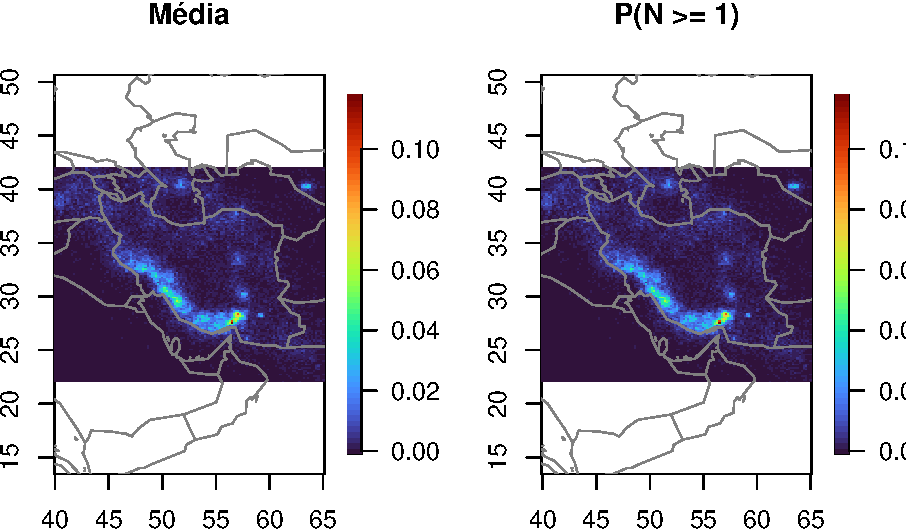
\includegraphics{relatorio_1_files/relatorio_1_files/figure-latex/mapa_pred_unico-1.pdf}

\hypertarget{usando-os-theta-bootstrap}{%
\subsection{\texorpdfstring{Usando os \(\theta\)
\emph{bootstrap}}{Usando os \textbackslash theta bootstrap}}\label{usando-os-theta-bootstrap}}

Quando usamos os valores de vários \(\hat{\theta}^{(b)}\) estimados por
meio de um \emph{bootstrap}, aumentamos a incerteza presente na
predição, mas os resultados são apresentados da mesma maneira. Teremos
que a predição temporal será:

\begin{verbatim}
##   bin_inicio  bin_fim media mediana p025 p975
## 1   13873.35 13903.35 4.706       4    1   13
## 2   13903.35 13933.35 4.981       4    0   12
## 3   13933.35 13963.35 4.800       4    0   12
## 4   13963.35 13993.35 4.892       4    0   12
## 5   13993.35 14023.35 5.052       5    1   13
## 6   14023.35 14053.35 4.889       4    0   12
## 7   14053.35 14083.35 4.925       4    0   13
\end{verbatim}

Neste caso, o valor médio por mês é um pouco menor do que no caso
anterior, provavelmente devido à quantidade de simulações em que
\(\hat{\theta}^{(b)}\) possui valores que diminuem a intensidade
condicional. De maneira similar, teremos que espacialmente:

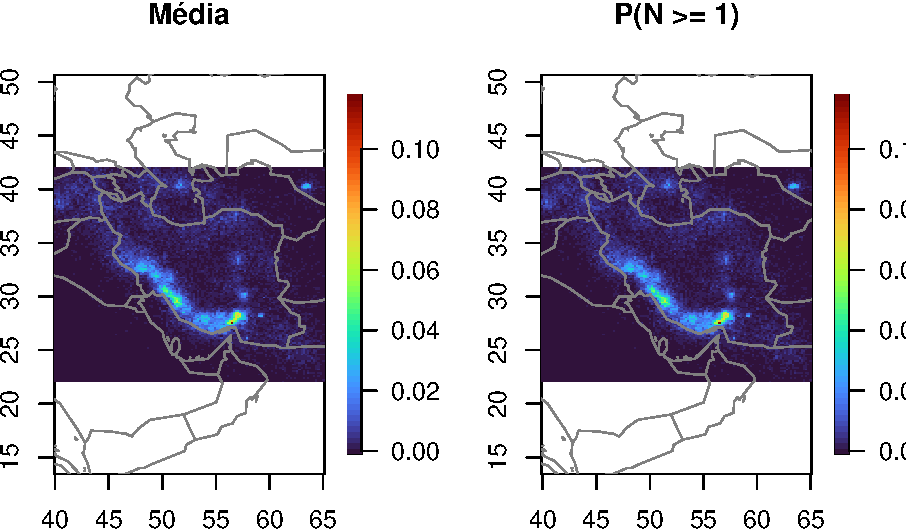
\includegraphics{relatorio_1_files/relatorio_1_files/figure-latex/mapa_pred_boot-1.pdf}

\hypertarget{sensibilidade}{%
\section{Sensibilidade}\label{sensibilidade}}

Um dos principais problemas apontados pelo autor, é que a função
\texttt{etas} é extremamente sensível à escolha de chute inicial para os
parâmetros. Para verificar se o mesmo ocorre com o método proposto, foi
realizado um estudo de sensibilidade, variando o valor inicial de
\(\theta\) em cada iteração.

Os catálogos foram contruídos usando a função
\texttt{simular_catalogo_etas}, com
\(\theta = (A = 0.5, \alpha = 1.5, c = 0.25, p = 1.5, D = 0.1, q = 2, \gamma = 0.1)\),
considerando \(m_{0} = 4.5\) e \(b = 1.5\), usando
\texttt{set.seed(123)}. Dois cenários de tamanho de amostra foram
explorados, primeiramente usando \texttt{T_max = 3650}, e posteriormente
usando \texttt{T_max = 5000}, para verificar se o tamanho de catálogo
influencia no resultado final.

Duas metodologias são usadas para variar os parâmetros: \textbf{OAT} e
\textbf{LHS}. No primeiro método, todos os parâmetros são mantidos no
valor verdadeiro (especificado anteriormente), e cada um é perturbado de
maneira individual separadamente (por isso \textbf{OAT} - \emph{One At
Time}). Cada parâmetro varia entre \(\frac{1}{4}\) do valor real até 2
vezes o valor real, ao longo de uma sequência igualmente espaçada com 10
valores (menos os parâmetros \(p\) e \(q\) que precisam ser maiores do
que 1, de modo que seus valores são determinados por
\(\theta_{variavel} = 1 + (\theta_{verdadeiro} - 1) \times \mathrm{multiplicador}\)).
Assim, são criados 70 pontos de partida distintos, cada um variando
apenas um parâmetro dentre os 7 possíveis.

Porém, não é usual que todos os parâmetros sejam conhecidos a menos de
um deles. Para isso um segundo método foi implementado, em que os
valores de todos os parâmetros são perturbados conjuntamente usando
amostragem por hipercubo latino (\textbf{LHS} - \emph{Latin Hypercube
Sampling}), que funciona da seguinte forma: para \(n\) pontos de partida
em \(k\) parâmetros, cada uma das \(k\) dimensões é dividida em \(n\)
faixas e cada uma é usada exatamente uma vez, garantindo cobertura
equilibrada do espaço paramétrico multidimensional com menos pontos do
que um fatorial completo. Aqui, foram utilizadas 50 pontos de partida
distintos.

Para fins de visualização, as primeiras e as últimas entradas da matriz
de \emph{design} dos pontos iniciais é dada por:

\begin{verbatim}
##               A     alpha          c        p          D        q      gamma
##  [1,] 0.1250000 1.5000000 0.25000000 1.500000 0.10000000 2.000000 0.10000000
##  [2,] 0.2222222 1.5000000 0.25000000 1.500000 0.10000000 2.000000 0.10000000
##  [3,] 0.3194444 1.5000000 0.25000000 1.500000 0.10000000 2.000000 0.10000000
##  [4,] 0.4166667 1.5000000 0.25000000 1.500000 0.10000000 2.000000 0.10000000
##  [5,] 0.5138889 1.5000000 0.25000000 1.500000 0.10000000 2.000000 0.10000000
##  [6,] 0.6111111 1.5000000 0.25000000 1.500000 0.10000000 2.000000 0.10000000
##  [7,] 0.7083333 1.5000000 0.25000000 1.500000 0.10000000 2.000000 0.10000000
##  [8,] 0.8055556 1.5000000 0.25000000 1.500000 0.10000000 2.000000 0.10000000
##  [9,] 0.9027778 1.5000000 0.25000000 1.500000 0.10000000 2.000000 0.10000000
## [10,] 1.0000000 1.5000000 0.25000000 1.500000 0.10000000 2.000000 0.10000000
## [11,] 0.6904647 3.0223080 0.07871798 1.338943 0.17249901 3.263291 0.04664732
## [12,] 0.3847757 1.3549030 0.28263245 1.233542 0.07745238 1.716240 0.07775635
## [13,] 0.1514160 1.0519954 0.31828567 1.492741 0.10117601 4.031965 0.22253082
## [14,] 0.8174373 0.4936352 0.11190258 2.019102 0.12204129 4.919364 0.07256729
## [15,] 1.2033701 4.7613038 0.30294915 1.162736 0.14133057 1.278643 0.14781675
## [16,] 0.9378407 0.9911100 0.93603471 2.045750 0.11664497 2.547733 0.30019096
## [17,] 0.7028772 4.5150162 0.47682866 1.151835 0.21917077 4.781158 0.02820848
## [18,] 1.9895430 2.2008551 0.13038995 1.211918 0.19582538 4.285333 0.24764748
## [19,] 0.8814421 1.5135764 0.66672297 2.715024 0.03073185 1.464841 0.10944940
## [20,] 0.1760598 0.4074005 0.19105242 1.270562 0.20691142 2.253528 0.10165796
\end{verbatim}

Note que nas primeiras 10 linhas, todos os parâmetros são fixos, e
muda-se apenas o valor de \(A\), enquanto que nas 10 últimas, todos os
parâmetros variam conjuntamente.

\hypertarget{resultados-para}{%
\subsection{\texorpdfstring{Resultados para
\texttt{T_max = 3650}}{Resultados para }}\label{resultados-para}}

Primeiramente, considerando um catálogo de 10 anos (3.650 dias), vejamos
os valores sumarizados de cada uma das colunas, sua amplitude e
desvios-padrão associados, para os 70 valores amostrados via
\textbf{OAT}:

\begin{verbatim}
## [1] "Sumário:"
\end{verbatim}

\begin{verbatim}
##                 A    alpha         c        p         D        q     gamma
## Min.    0.4716051 1.560100 0.3694916 1.673278 0.1511463 2.400953 0.1551788
## 1st Qu. 0.4716347 1.560223 0.3696242 1.673423 0.1513630 2.401914 0.1560600
## Median  0.4716519 1.560273 0.3697716 1.673700 0.1514276 2.402597 0.1562351
## Mean    0.4716511 1.560268 0.3697607 1.673617 0.1514109 2.402400 0.1562806
## 3rd Qu. 0.4716727 1.560304 0.3698830 1.673787 0.1514603 2.402750 0.1564843
## Max.    0.4717092 1.560468 0.3702657 1.674062 0.1515776 2.403382 0.1577166
\end{verbatim}

\begin{verbatim}
## [1] "Amplitude:"
\end{verbatim}

\begin{verbatim}
##            A        alpha            c            p            D            q        gamma 
## 0.0001041406 0.0003682838 0.0007741232 0.0007840945 0.0004312994 0.0024286965 0.0025377542
\end{verbatim}

\begin{verbatim}
## [1] "Desvios-Padrão:"
\end{verbatim}

\begin{verbatim}
##            A        alpha            c            p            D            q        gamma 
## 2.325216e-05 6.816715e-05 1.547667e-04 1.993249e-04 8.035295e-05 5.315653e-04 4.364740e-04
\end{verbatim}

E para os 50 valores amostrados via \textbf{LHS}:

\begin{verbatim}
## [1] "Sumário:"
\end{verbatim}

\begin{verbatim}
##                 A    alpha         c        p         D        q     gamma
## Min.    0.4715612 1.559883 0.3694882 1.673276 0.1508821 2.400061 0.1533677
## 1st Qu. 0.4716149 1.560172 0.3696382 1.673432 0.1512635 2.401404 0.1556857
## Median  0.4716520 1.560320 0.3697081 1.673571 0.1513572 2.401902 0.1565674
## Mean    0.4716475 1.560330 0.3697447 1.673584 0.1513434 2.401939 0.1567074
## 3rd Qu. 0.4716750 1.560421 0.3698791 1.673729 0.1514373 2.402555 0.1573568
## Max.    0.4717313 1.560877 0.3700670 1.674014 0.1516279 2.403415 0.1606347
\end{verbatim}

\begin{verbatim}
## [1] "Amplitude:"
\end{verbatim}

\begin{verbatim}
##            A        alpha            c            p            D            q        gamma 
## 0.0001700673 0.0009940144 0.0005787770 0.0007381550 0.0007457352 0.0033535276 0.0072670730
\end{verbatim}

\begin{verbatim}
## [1] "Desvios-Padrão:"
\end{verbatim}

\begin{verbatim}
##            A        alpha            c            p            D            q        gamma 
## 4.557061e-05 2.221641e-04 1.700534e-04 1.956113e-04 1.598672e-04 7.774207e-04 1.580219e-03
\end{verbatim}

Podemos notar que, essencialmente, todos os valores iniciais resultaram
em valores finais extremamente semelhantes, com uma variabilidade muito
baixa, em ambos os métodos de amostragem. Assim, podemos constatar que o
método proposto não é sensível à escolha de parâmetros iniciais. Além
disso, é possível verificar o quanto cada parâmetro foi estimado de
maneira errônea, por meio do erro relativo médio (dado por
\(\frac{\theta_{est} - \theta_{ver}}{\theta_{ver}}\)) de cada parâmetro:

\begin{verbatim}
## [1] "Erro relativo médio:"
\end{verbatim}

\begin{verbatim}
##           A       alpha           c           p           D           q       gamma 
## -0.05670080  0.04019594  0.47901610  0.11573554  0.51382755  0.20110385  0.56458412
\end{verbatim}

Podemos verificar também, além disso, o erro quadrático médio de cada um
dos parâmetros:

\begin{verbatim}
## [1] "Erro quadrático médio:"
\end{verbatim}

\begin{verbatim}
##            A        alpha            c            p            D            q        gamma 
## 0.0008037463 0.0036353794 0.0143410519 0.0301381476 0.0026402027 0.1617714962 0.0031887257
\end{verbatim}

Apesar do erro quadrático médio baixo, o erro relativo médio mostra que
alguns parâmetros sofrem desvios significativos de suas estimativas
verdadeiras (notadamente \(c\), \(D\) e \(\gamma\), com desvios próximos
a 50\% do valor original).

\hypertarget{resultados-para-1}{%
\subsection{\texorpdfstring{Resultados para
\texttt{T_max = 5000}}{Resultados para }}\label{resultados-para-1}}

Vejamos se o aumento no tamanho do catálogo tem influência nos
resultados da sensibilidade. Primeiramente, para os 70 valores
amostrados via \textbf{OAT}:

\begin{verbatim}
## [1] "Sumário:"
\end{verbatim}

\begin{verbatim}
##                 A    alpha         c        p         D        q     gamma
## Min.    0.4479013 1.628697 0.3232357 1.642685 0.1014786 2.063349 0.1764024
## 1st Qu. 0.4479337 1.629242 0.3234649 1.642937 0.1015184 2.063562 0.1786717
## Median  0.4479937 1.629410 0.3236840 1.643199 0.1015350 2.063808 0.1792202
## Mean    0.4479966 1.629394 0.3236229 1.643135 0.1015351 2.063775 0.1791812
## 3rd Qu. 0.4480542 1.629566 0.3237436 1.643275 0.1015467 2.063969 0.1796909
## Max.    0.4481974 1.629784 0.3238522 1.643488 0.1016841 2.064161 0.1803243
\end{verbatim}

\begin{verbatim}
## [1] "Amplitude:"
\end{verbatim}

\begin{verbatim}
##            A        alpha            c            p            D            q        gamma 
## 0.0002960957 0.0010876146 0.0006165452 0.0008029045 0.0002054359 0.0008119545 0.0039218535
\end{verbatim}

\begin{verbatim}
## [1] "Desvios-Padrão:"
\end{verbatim}

\begin{verbatim}
##            A        alpha            c            p            D            q        gamma 
## 6.562349e-05 1.963373e-04 1.559092e-04 2.063120e-04 2.760782e-05 2.340688e-04 6.731426e-04
\end{verbatim}

E para os 50 valores amostrados via \textbf{LHS}:

\begin{verbatim}
## [1] "Sumário:"
\end{verbatim}

\begin{verbatim}
##                 A    alpha         c        p         D        q     gamma
## Min.    0.4478161 1.628077 0.3232724 1.642562 0.1013986 2.063230 0.1737633
## 1st Qu. 0.4479492 1.629165 0.3233820 1.642833 0.1014995 2.063461 0.1787189
## Median  0.4480149 1.629357 0.3234859 1.642949 0.1015189 2.063670 0.1790238
## Mean    0.4480196 1.629316 0.3234941 1.642972 0.1015432 2.063680 0.1788397
## 3rd Qu. 0.4480579 1.629514 0.3235890 1.643089 0.1015715 2.063868 0.1796620
## Max.    0.4483340 1.630199 0.3238772 1.643427 0.1018351 2.064131 0.1813168
\end{verbatim}

\begin{verbatim}
## [1] "Amplitude:"
\end{verbatim}

\begin{verbatim}
##            A        alpha            c            p            D            q        gamma 
## 0.0005179637 0.0021222732 0.0006047792 0.0008644889 0.0004365495 0.0009010508 0.0075534393
\end{verbatim}

\begin{verbatim}
## [1] "Desvios-Padrão:"
\end{verbatim}

\begin{verbatim}
##            A        alpha            c            p            D            q        gamma 
## 1.109267e-04 4.308769e-04 1.472093e-04 1.866259e-04 9.621445e-05 2.391969e-04 1.617971e-03
\end{verbatim}

Aqui, temos o comportamento semelhante aos resultados obtidos com um
catálogo de 10 anos, de alta consistência na estimação de todos os
parâmetros, não sendo sensível à escolha do chute inicial. Vejamos
porém, seu comportamento em relação aos erros de estimação:

\begin{verbatim}
## [1] "Erro relativo médio:"
\end{verbatim}

\begin{verbatim}
##           A       alpha           c           p           D           q       gamma 
## -0.10398760  0.08624100  0.29427693  0.09537783  0.01538464  0.03186761  0.79038922
\end{verbatim}

\begin{verbatim}
## [1] "Erro quadrático médio:"
\end{verbatim}

\begin{verbatim}
##            A        alpha            c            p            D            q        gamma 
## 2.703363e-03 1.673450e-02 5.412459e-03 2.046814e-02 2.371107e-06 4.062235e-03 6.248509e-03
\end{verbatim}

É possível perceber que os erros relativos de \(A\) e \(\alpha\)
mantiveram-se pequenos, os de \(c\) e \(p\) diminuíram consideravelmente
e que os de \(D\) e \(q\) reduziram drasticamente. O único que aumentou
significativamente o erro relativo foi \(\gamma\), com quase 80\% de
erro relativo. Porém, esses parâmetros (\(D,q\) e \(\gamma\)) são
altamente correlacionados, e a estimação conjunta de todos é complicada.
A nível de comparação, vejamos-os conjuntamente:

\begin{verbatim}
##               A alpha     c     p     D     q gamma
## T = 3650 -0.057 0.040 0.479 0.116 0.514 0.201 0.565
## T = 5000 -0.104 0.086 0.294 0.095 0.015 0.032 0.790
\end{verbatim}

Dito isso, o ajuste foi extremamente satisfatório, e mostrou-se
consistente independentemente do tamanho amostral, com melhora no erro
conforme o tamanho do catálogo aumenta. Podemos comprovar isso
observando o \emph{background rate} médio estimado em cada caso:

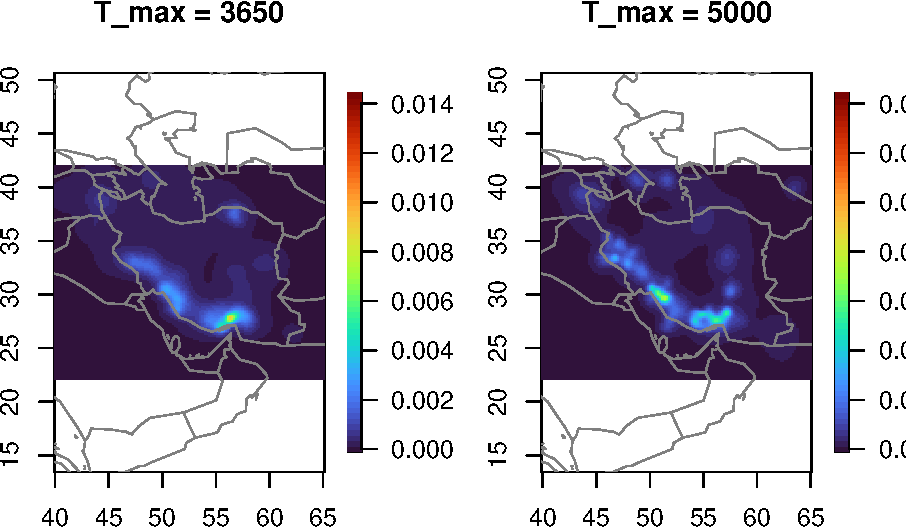
\includegraphics{relatorio_1_files/relatorio_1_files/figure-latex/backgrounds_medios-1.pdf}

Quando comparamos com o \emph{background rate} verdadeiro usado para a
simulação, que é:

\begin{center}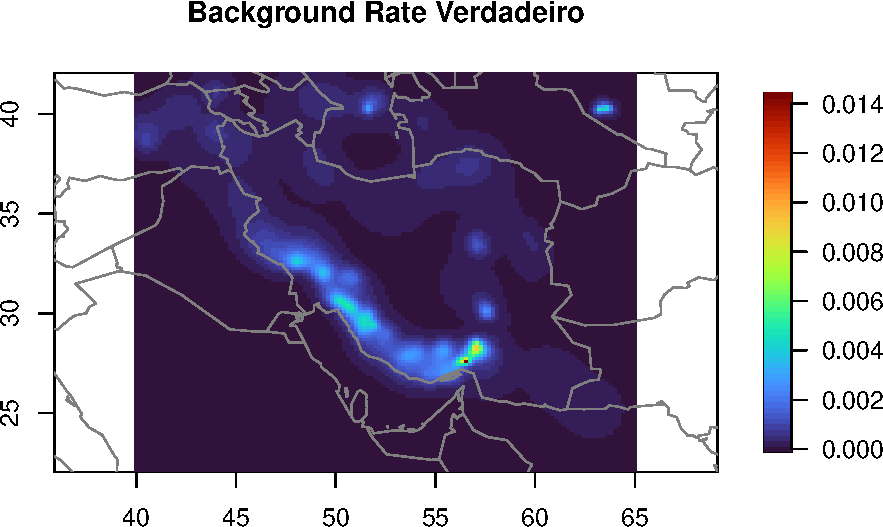
\includegraphics{relatorio_1_files/figure-latex/background_real-1} \end{center}

Vemos que o \emph{background rate} médio do catálogo maior é mais
semelhante ao real, o que pode justificar o menor erro nos estimadores.





\newpage
\singlespacing
\bibliography{ref.bib}

\end{document}
